\documentclass[10pt,letterpaper]{article}
\usepackage[margin=0.75in,top=0.65in,bottom=0.7in]{geometry}
\usepackage[T1]{fontenc}
\usepackage{helvet}
\renewcommand{\familydefault}{\sfdefault}
\renewcommand{\topfraction}{0.85}\renewcommand{\textfraction}{0.1}\renewcommand{\floatpagefraction}{0.8}
\usepackage{microtype}
\usepackage{amsmath,amssymb}
\usepackage{graphicx}
\usepackage{xcolor}
\usepackage{enumitem}
\usepackage[font=small,labelfont=bf,skip=2pt]{caption}
\usepackage[skins,breakable]{tcolorbox}
\usepackage{titlesec}
\usepackage[hidelinks]{hyperref}
\usepackage{url}
\usepackage[section]{placeins}

% Agent-drafted prose is wrapped in \cl{...}. Identity by default.
% To color it, replace the next line with: \newcommand{\cl}[1]{{\color{teal}#1}}
\newcommand{\cl}[1]{#1}

\setlist{nosep,leftmargin=1.1em,topsep=1pt}
\titleformat{\section}{\large\bfseries}{\thesection}{0.5em}{}
\titlespacing*{\section}{0pt}{7pt}{2pt}
\setlength{\parindent}{0pt}
\setlength{\parskip}{2pt}
\setlength{\textfloatsep}{6pt plus 2pt}
\setlength{\floatsep}{6pt plus 2pt}
\setlength{\intextsep}{6pt plus 2pt}
\urlstyle{same}

\newtcolorbox{where}{enhanced,colback=gray!6,colframe=gray!45,boxrule=0.4pt,arc=1pt,
  left=3pt,right=3pt,top=1pt,bottom=1pt,fontupper=\footnotesize\raggedright,before skip=3pt,after skip=3pt}
\newcommand{\asked}[1]{\textbf{Asked} (plan file): \emph{``#1''}\par}
\newcommand{\hd}[1]{\textbf{#1}\par}

\begin{document}

{\Large\bfseries Peeling the onion: progress to 2026-11-15}\par
{\normalsize Mehdi Foroozandeh}\quad{\small 2026-11-10 to 2026-11-15. Each section answers one part of the plan file \emph{peeling the onion}.}

\begin{tcolorbox}[enhanced,colback=orange!6,colframe=orange!60!black,boxrule=0.5pt,arc=1pt,left=3pt,right=3pt,top=1pt,bottom=1pt,fontupper=\small,before skip=4pt,after skip=4pt]
\cl{\begin{itemize}
\item All model scores are screening scores (pairs on 16 of the 256 regions). The architecture tiers are provisional: untuned, equal windows not equal compute. A tuning round is queued.
\item The correction metric is under review: scrambled covariates \emph{raised} all-pair gap closed at the U-Net (+0.101, seed range 0.052).
\item 10 of 38 named ablations are fully tested; the output-side depth arm has 1 seed. Whether the counterfactual views help imputation is untested; the ablation is queued.
\item The extended dataset is a catalog only; the balanced split is not started. Nibi compute has been down since 13:10 UTC on 2026-11-15.
\end{itemize}}
\end{tcolorbox}

\begin{where}
GitHub \texttt{mehdiforoozandeh/CANDII}, branch \path{implementation/t152-peeling-the-onion} (draft PR 61); vault paths are relative to the repository.
Nibi \texttt{O = }\path{/project/def-maxwl/mforooz/ONION} (all paths checked with \texttt{ls -ld} on 2026-11-15; group \texttt{def-maxwl} can read them).
Fir: \path{/project/def-maxwl/mforooz/ONION} holds a partial copy (Globus, 2026-11-14); copy not verified complete.
\end{where}

%=====================================================================
\section{Sources of variation}
\asked{there are different axes and sources of variation in the data that we are working with}
\cl{\hd{Answer so far}
\begin{itemize}
\item Data processing: every EIC experiment has a base view and 8 designed views (Fig.~\ref{fig:onion}).
\item Read sampling: every view has two pseudoreplicate halves (random read halves); 778 half pairs enter the layers.
\item Data generation: only the isogenic replicates (same-donor biological replicates) of the EIC give pairs, 219 of them. Lab, platform and antigen are not separated.
\item Biological: cell type from 2,911 pairs of different cell types (mixed with donor and lab); position by region stratum and scale; assay per assay. Population: not addressed.
\end{itemize}
\hd{Open}
\begin{itemize}
\item A lab layer needs second experiments of one cell and assay. The blind set is 100\% paired-end and 94\% from one lab, and the views imitate only paired-end to single-end and long to short reads.
\end{itemize}}

\begin{figure}[!ht]
\centering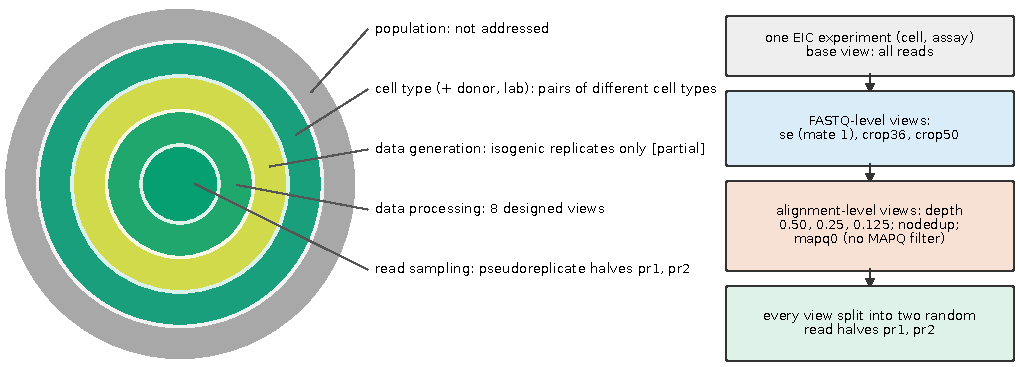
\includegraphics[width=0.9\textwidth]{figs/fig1_onion_views.pdf}
\caption{\cl{Each layer of the onion except population has a data view: designed processing views and pseudoreplicate halves of every experiment, isogenic replicates, and pairs of cell types.}}
\label{fig:onion}
\end{figure}

\begin{where}
\path{O/tables/eic_v1/} (\path{measurements.tsv}, \path{pairs.tsv}, \path{withheld.tsv}); counts and halves \path{/scratch/mforooz/onion/measurements/<id>/{counts,pr1,pr2}.h5}%DAG
; archive \path{/nearline/def-maxwl/mforooz/onion/eic_v1/}.
Vault: \path{cruxvault/results/t170/withheld_design.md}, \path{cruxvault/results/t183/DATASET_EIC_V1.md}.
\end{where}

%=====================================================================
\section{Objectives}
\asked{impute across different axes of biological variation \ldots\ correct artifacts \ldots\ calibrated aleatoric uncertainty}
\cl{\hd{Answer so far: one lead term per goal, each on 0 to 1}
\begin{itemize}
\item Imputation: specific variance recovered above the noise floor, $1-(E_{sp}-N)/(V_{sp}-N)$ (cell-type-specific error, variance, pseudoreplicate floor).
\item Correction: gap closed on never-trained view pairs; 0 = depth-only scaling, 1 = the oracle floor (half the mean $|$pr1 $-$ pr2$|$ of the target). CRPS (error of a whole predictive distribution) is the score.
\item Uncertainty: $1-\mathrm{PIT}_{\text{model}}/\mathrm{PIT}_{\text{marginal NB}}$, with PIT the predicted CDF at the observed count.
\item Composite $=0.5\,$imputation$\,+\,0.25\,$correction$\,+\,0.25\,$uncertainty, terms clipped to $[0,1]$; an arm wins only by more than 2 seed ranges over 3 seeds.
\end{itemize}
\hd{Open}
\begin{itemize}
\item On 84 of the 102 headline pairs one side keeps duplicates, so source and target can share fragments; only 18 pairs are clean. A clean-pair correction term is the candidate fix.
\end{itemize}}
\begin{where}
\path{tools/onion_eval/select_rule.py}; vault \path{cruxvault/INSTRUCTIONS/peeling_the_onion/}\texttt{onion eval protocol.md}, \path{cruxvault/results/oracle_floor/ORACLE_FLOOR.md}.
\end{where}

%=====================================================================
\section{Eval: the onion, peeled on real data}
\asked{dividing the total variance by its different components and finally what can't be modelled}
\cl{\hd{Law of total variance} With count $Y$, depth $D$ and depth-free rate $r$, $Y\mid r\sim\mathrm{Poisson}(Dr)$ (theory):
\[ \mathrm{Var}(Y)=\underbrace{D\,\mathbb{E}[r]}_{\text{read sampling}}+\underbrace{D^2\,\mathrm{Var}(r)}_{\text{all layers above sampling}} . \]
Layers are differences of pair values: halves (sampling), isogenic minus halves (replicate), other cell type minus isogenic (cell type).

\hd{Offset off versus offset on (Fig.~\ref{fig:layers})}
\begin{itemize}
\item Offset off: layers on log1p counts at one thinned depth, so the Poisson term sits in every layer. Sampling is 76\% to 97\% of the three layers; replicate 0.1\% to 6\%; cell type up to 23\%.
\item Offset on: layers of the rate $r=e^{\eta}$ (mean $=D\,e^{\eta}$), with the Poisson term removed exactly by factorial moments, $\mathbb{E}[Y(Y-1)]=D^2\mathbb{E}[r^2]$.
\item Changed on real data: thinning to 1/4 depth moved the offset-on layers by at most 10\%, but cut the offset-off cell-type share by 8\% to 63\%.
\item Changed: the replicate share of the layers above sampling is 0.24 for H3K27ac offset on, against 0.07 offset off.
\item Changed: the ChIP control has a cell-type layer, 0.38 [0.23, 0.54] of its sampling-free variance, where log1p gave $-0.002$.
\end{itemize}
\textbf{Answer:} offset on is more sensitive to sources other than pseudoreplicate (read-sampling) noise, and it is depth-free. \textbf{Limits:} peak bins dominate the estimates; assays with 8 to 12 isogenic pairs have wide intervals; no model is scored offset on yet.}

\begin{figure}[!ht]
\centering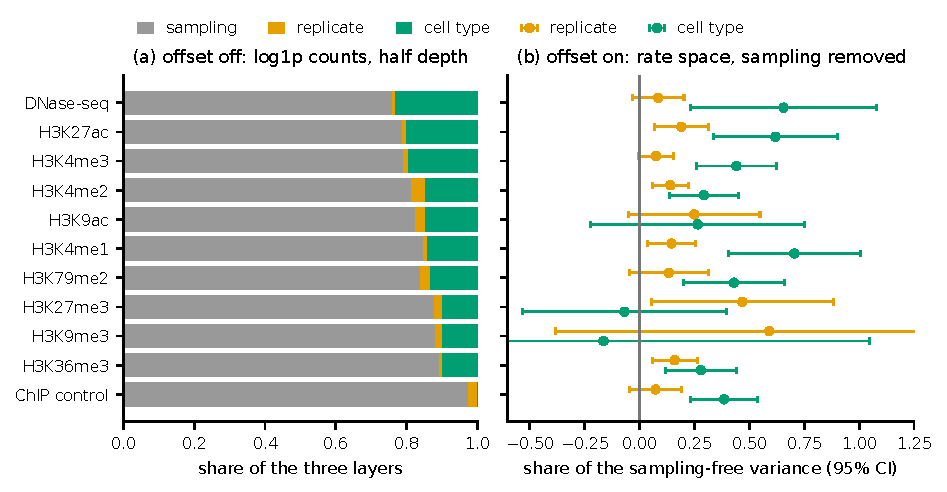
\includegraphics[width=0.86\textwidth]{figs/fig4_layers.pdf}
\caption{\cl{Offset off, read sampling fills 76\% to 97\% of the per-bin variance; offset on, sampling is removed and the replicate and cell-type layers are large. Panel b: 95\% intervals over cells; H3K9me3 intervals extend beyond the axis.}}
\label{fig:layers}
\end{figure}

\cl{\hd{Benchmark and other methods (Fig.~\ref{fig:base})}
\begin{itemize}
\item Frozen benchmark: 256 regions of 409.6 kb; 63 imputation items; 1,480 correction pairs, 102 of them never-trained headline pairs.
\item Best training-free correction: the position average closes 0.258 [0.192, 0.373] of the gap to the oracle floor.
\item AlphaGenome 2, on 11 tracks in 9 cells unseen by it and by us: recalibrated $r_{\text{spec}}$ (correlation after removing the training mean) 0.438, against 0.222 for the position average and 0.333 [0.276, 0.382] for the noise floor.
\end{itemize}
\hd{Open}
\begin{itemize}
\item Resolution, breakdown by artifact source, and by genome subset are not yet scored for models; AlphaGenome 2 has no miniCANDI row yet.
\end{itemize}}

\begin{figure}[!ht]
\centering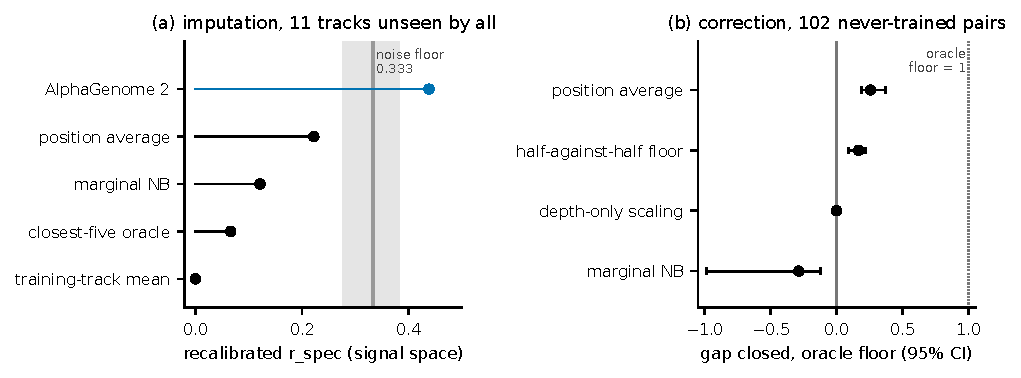
\includegraphics[width=0.8\textwidth]{figs/fig5_baselines.pdf}
\caption{\cl{AlphaGenome 2 leads every training-free reference on unseen tracks; the position average is the correction baseline to beat. Panel b: 95\% intervals over cells, 256 regions.}}
\label{fig:base}
\end{figure}

\begin{where}
\path{O/eval/eic_v1/} (\path{evalset.json}, \path{evalset_p16.json}, \path{baselines/}, \path{layers_t305/}); AlphaGenome 2 \path{O/ag2/} (\path{cache/}, \path{pack/eic_v1/}, \path{scores/eic_v1/baselines_fl/headline/}).
Vault: \path{cruxvault/results/t305/LAYERS_REAL.md}, \path{cruxvault/results/eta_space/LAYERS_ETA.md}, \path{THEORY.md}, \path{cruxvault/results/t307/BASELINES.md}, \path{cruxvault/results/t308/AG2_VS_BASELINES.md}.
\end{where}

%=====================================================================
\section{Data}
\asked{we are collecting a new extended dataset; we are retiring EED; we are updating our EIC dataset}
\cl{\hd{Answer so far}
\begin{itemize}
\item Updating EIC: done. Rebuilt from reads with the standard ENCODE pipelines, checked by accession (check PASS): 2,740 measurements.
\item Present: 249 of 267 training tracks (the 18 absent are DNase-seq), 42 of 45 validation, 37 of 40 controls; so DNase-seq is not imputation-scorable yet.
\item Retiring EED: done; this run does not use it.
\item Extended dataset: ENCODE catalog and census only; the balanced Cell, Assay, Measurement split is not started.
\end{itemize}}
\begin{where}
\path{O/eic/} (build list, \path{accession_ledger.tsv}%DAG2
, \path{tail/}); \path{O/catalog/encode/}; earlier single-end reprocessing of the blind tracks \path{/project/def-maxwl/mforooz/EIC_REPRO/003_pipeline/results/}.
Vault: \path{cruxvault/results/t183/DATASET_EIC_V1.md}, \path{cruxvault/results/t156/CENSUS.md}.
\end{where}

%=====================================================================
\section{Did the counterfactual views help?}
\asked{show where and if adding counterfactual data (augmenting EIC) actually helps}
\cl{\hd{Answer so far}
\begin{itemize}
\item The views made the correction task: the 1,480 correction pairs and the 102 never-trained headline pairs exist only because of them; the halves give the sampling layer and the imputation noise floor.
\item Correction has most room where the target is deeper: depth-only scaling trails the half floor by a CRPS gap of 0.182 to 0.234 on depth-increasing pairs that also change processing, against 0.081 [0.049, 0.125] on pure depth-increasing pairs.
\item Every architecture closed more of the gap than the position average (0.235): from 0.291 (Perceiver IO) to 0.576 (conv autoencoder).
\item By view change, only the pointwise MLP has a breakdown: crop pairs 0.582 (range 0.034), mapq+nodedup pairs 0.420 (range 0.017). No such breakdown exists for the U-Net or the conv autoencoder.
\item Untested: whether training on the views helps imputation or calibration, and which views carry it, because every model trained on all views. An ablation (U-Net on base view only, all views without cross-view pairs, base plus depth, base plus FASTQ-level, base plus alignment-level; 3 seeds each) is queued, no result.
\end{itemize}}
\begin{where}
\path{O/tables/eic_v1/} (\path{measurements.tsv}, \path{pairs.tsv}, \path{withheld.tsv}); \path{/scratch/mforooz/onion/measurements/}%DAG3
.
Vault: \path{cruxvault/results/t307/correction_headroom.tsv}, \path{cruxvault/results/oracle_floor/per_knob_p16.tsv}, \path{cruxvault/results/metrics_screening/scores_ladder.md}.
\end{where}

%=====================================================================
\section{miniCANDI: the prototype}
\asked{miniCANDI is the prototype and we move on to CANDI when we are sure that miniCANDI prototype is well defined and working}
\cl{\hd{Answer so far}
\begin{itemize}
\item Built as planned: inputs $X$, $S$, $C$, $C'$; an NB per assay and 25 bp bin with mean $=\text{depth}'\times2^{\eta}$; NB loss on masked and on corrected assays. Six architectures of about 1.0 M parameters, 80,000 windows, 3 seeds.
\item Three composite tiers (Fig.~\ref{fig:ladder}): conv autoencoder 0.502 (range 0.031) and conv plus attention 0.493 (0.033); axial transformer, U-Net, pointwise MLP 0.444 to 0.469; Perceiver IO 0.261 (0.052).
\item The U-Net recovers the most specific variance, 0.440 (0.013), but closes the least gap of the top five, 0.298 (0.052).
\item Covariates: scrambling them at the U-Net lowered specific variance by 0.029 (0.013) but raised all-pair gap closed by 0.101 (0.052).
\item Depth (Fig.~\ref{fig:arms}): hiding it on the input side lowered the composite from 0.444 (0.030) to 0.382 (0.009); only hiding it on both sides and in the input transform collapsed calibration (uncertainty term 0.600 to $-0.099$).
\item Training regions: no selection rule beat uniform sampling (best +0.009, range 0.029).
\end{itemize}
\hd{Open}
\begin{itemize}
\item Provisional tiers: no tuning, no held-out loss. The queued tuning round has 42 trial runs over five architectures under one protocol (choice on held-out loss only), after 36 runs of a first round; the pointwise MLP trials wait for the GPU queue. Compute can move to Fir.
\item Input-side depth hiding \emph{raised} clean-pair gap closed (0.519 to 0.601); no tested explanation yet. The output-side arm has 1 seed (0.462).
\item Coverage: 10 of the 38 ablations the plan names are fully tested, 7 partial, 21 untested (Fig.~\ref{fig:cov}).
\end{itemize}}

\begin{figure}[!ht]
\centering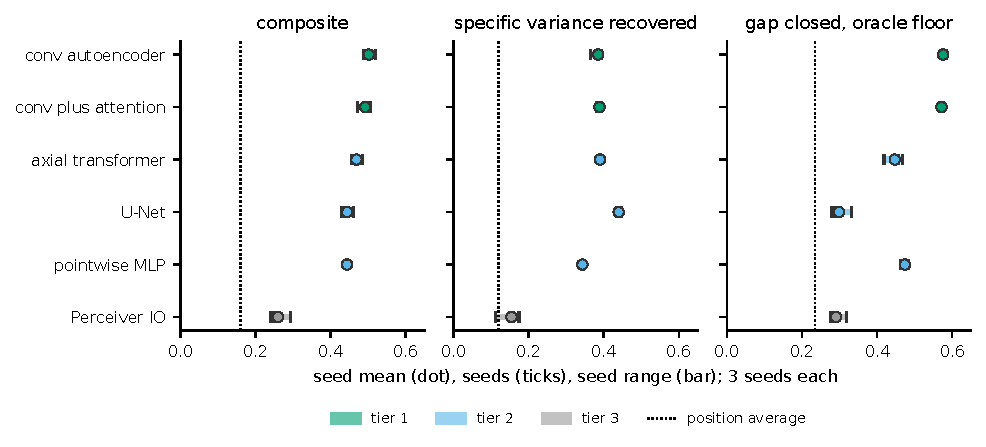
\includegraphics[width=0.8\textwidth]{figs/fig7_ladder.pdf}
\caption{\cl{Three tiers survive the seed test: the conv models lead the composite, the U-Net leads specific variance but closes the least gap, and Perceiver IO is last under this untuned recipe.}}
\label{fig:ladder}
\end{figure}

\begin{figure}[!ht]
\centering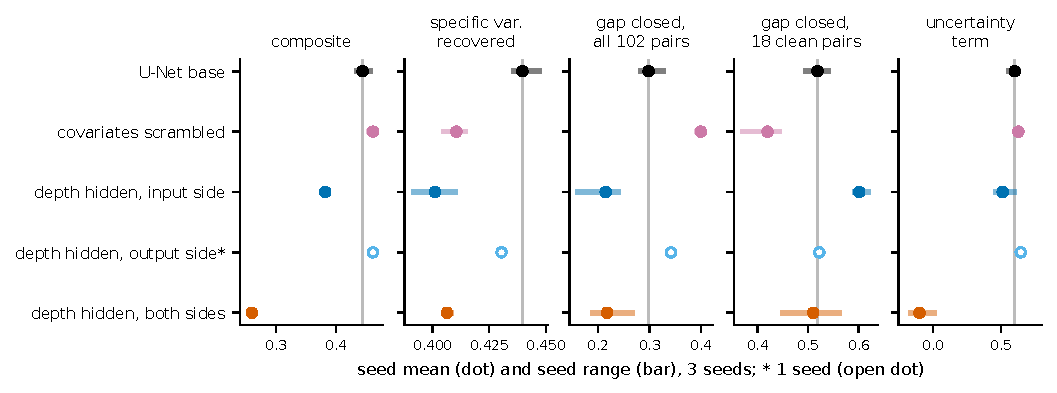
\includegraphics[width=0.78\textwidth]{figs/fig8_arms.pdf}
\caption{\cl{U-Net arms. Input-side depth hiding: specific variance fell 0.440 to 0.401 and clean-pair gap closed rose 0.519 to 0.601, both beyond the seed ranges; all-pair gap closed (0.298 to 0.215) and the uncertainty term (0.600 to 0.511) stayed inside the seed ranges. Only hiding depth on both sides and in the input transform collapsed the uncertainty term ($-0.099$). Scrambled covariates raised all-pair but lowered clean-pair gap closed. Grey line: base mean.}}
\label{fig:arms}
\end{figure}

\begin{figure}[!ht]
\centering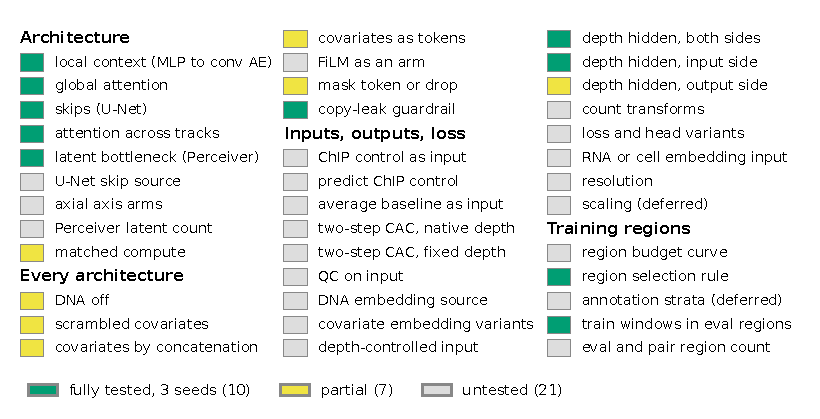
\includegraphics[width=0.7\textwidth]{figs/fig9_coverage.pdf}
\caption{\cl{Ten of the 38 named ablations are fully tested; most input, output and loss knobs are untested.}}
\label{fig:cov}
\end{figure}

\begin{where}
\path{O/runs/<run>/seed<k>/} (\path{run.json}, \path{log.jsonl}%DAG4
, \path{p16/scores.json}); predictions \path{/scratch/mforooz/onion/pred_store/}%DAG5
; code \path{/project/def-maxwl/mforooz/onion_kit/FC/}. Run folders \path{rung1_base} to \path{rung6_base} = pointwise MLP, conv autoencoder, conv plus attention, U-Net, axial transformer, Perceiver IO.
Vault: \path{cruxvault/results/metrics_screening/}, \path{cruxvault/results/ladder_audit/}\{\path{FAIR_CHANCE.md}, \path{COVERAGE.md}\}.
\end{where}

%=====================================================================
\section{Not started: scaling}
\asked{later on at scaling, we want to scale on three axes and observe the effects}
\cl{Not started, as the plan places it after a working prototype. The queued 160,000-window runs check the prototype, not scaling.}

\end{document}
